\chapter{实验过程}
上一个章节获取到了所有的数据之后, 下一步就是使用神经网络进行训练,分析结果。

\section{运行环境}

本课设使用的框架是tensorflow非GPU版本。\\
运行硬件环境使用neofetch得到结果如下:
\begin{Verbatim}[]
             ............                martin@martin-PC 
         .';;;;;.       .,;,.            ---------------- 
      .,;;;;;;;.       ';;;;;;;.         OS: Deepin 15.6 x86_64 
    .;::::::::'     .,::;;,''''',.       Model: 20BVA02ACD ThinkPad T450 
   ,'.::::::::    .;;'.          ';      Kernel: 4.15.0-21deepin-generic 
  ;'  'cccccc,   ,' :: '..        .:     Uptime: 11 hours 
 ,,    :ccccc.  ;: .c, '' :.       ,;    Packages: 2671 
.l.     cllll' ., .lc  :; .l'       l.   Shell: zsh 5.3.1 
.c       :lllc  ;cl:  .l' .ll.      :'   Resolution: 1366x768 
.l        'looc. .   ,o:  'oo'      c,   DE: Deepin 
.o.         .:ool::coc'  .ooo'      o.   WM: Mutter(DeepinGala) 
 ::            .....   .;dddo      ;c    Theme: Deepin [GTK2/3] 
  l:...            .';lddddo.     ,o     Icons: Deepin [GTK2/3] 
   lxxxxxdoolllodxxxxxxxxxc      :l      Terminal: tilix 
    ,dxxxxxxxxxxxxxxxxxxl.     'o,       CPU: Intel i5-5200U (4) @ 2.700GHz 
      ,dkkkkkkkkkkkkko;.    .;o;         GPU: Intel Integrated Graphics 
        .;okkkkkdl;.    .,cl:.           GPU: NVIDIA GeForce 940M 
            .,:cccccccc:,.               Memory: 3680MiB / 7677MiB 
\end{Verbatim}
\section{构建神经网络}
在实验的过程中间, 曾经尝试过使用CNN, 但是测试的时候发现的CNN的运行结果非常的慢
的, 所以放弃使用, 所以以下得到的结果所有的运行的使用的是相同网络模型, 只有当
数据的维度发生变化的时候, 才会自适应做出调整。 \ref{lab_table_1}和
\ref{lab_table_2}分别是Generator和Discriminator的网络的配置, 两个网络全部使用的是最简
单的全连接网络。

\begin{table}[htb]
\centering
\label{lab_table_1}
\begin{tabular}{c|c|c|c}
\hline\hline

\textbf{层} & \textbf{一} & \textbf{二} & \textbf{三} \\
\hline\hline
维度    & 噪音维度 100 & 100  300 & 300  图片维度\\
\hline
\hline\hline
\end{tabular}
\caption{Generator网络结构参数}
\end{table}


\begin{table}[htb]
\centering
\label{lab_table_2}
\begin{tabular}{c|c|c|c}
\hline\hline

\textbf{层} & \textbf{一} & \textbf{二} & \textbf{三} \\
\hline\hline
维度    & 图片维度  300 & 300 100  & 100 1\\
\hline
\hline\hline
\end{tabular}
\caption{Discriminator网络结构参数}
\end{table}

由于GAN的特殊性,构建网络的时候有几个需要注意的位置


\begin{itemize}
  \item 当训练D的时候, 中间包含了G生成的噪音数据,如果训练的时候不指定是哪一个
  变量列表, 那么在训练D的时候, 同时会修改G的参数。

  \item 在大多数的情况之下, G的实现是通过函数来实现, 如果调用两次该函数,得到的
  是两个网络, 但是为了让G生成数据和z 生成的数据经过的是同一个网络, 可以采用的
  方法tensorflow提供的resue\_variable函数, 或者让两个数据连接成为一个整体, 然后调
  用G的函数。
\end{itemize}



\section{完善备份和展示功能}
网络构建完成之后就可以了,但是实现更加多的辅助功能可以方便的自己的实验。\\
tensorflow提供了一个保存运行参数,在每一次循环的时候保存checkpoint, 当用于种种原
因实验中断的之后, 只要日志文件依旧存在,就可以继续之前的运行。

第二个是借用tensorboard工具, 更加容易的显示结果出来, 在数据准备阶段中间的数据
的截图就是全部来自于使用tensorboard 工具的截图。

\section{测试结果展示}
在制作的数据的时候, 本来以为所有的数据都是有比较好的结果, 但是实际上发现,有的
数据可以得到比较好的结果, 比如MNIST, 有的数据只是得到了数据的大体的特征,创建的
数据的最主要的特征已经完全消失了, 而有的数据得到的结果没有任何的意义, 完全看不
到生成的数据的含义所在。

\subsection{MNIST}
MNIST的测试效果相对于其他的数据的测试结果效果最佳, \ref{mnist-res-a}和
\ref{mnist-res-b}中间的数据的结果几乎可以原始的数据相同。
\begin{figure}[!hbt]
    \centering
    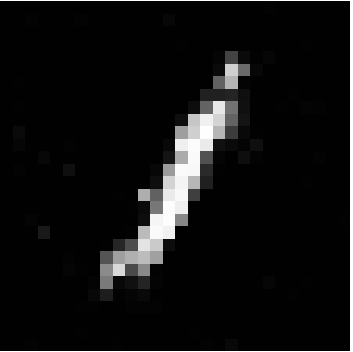
\includegraphics[width=0.3\linewidth]{pic/mnist-res-a.png}
    \caption{生成手写字1}
    \label{minist-res-a}
\end{figure}

\begin{figure}[!hbt]
    \centering
    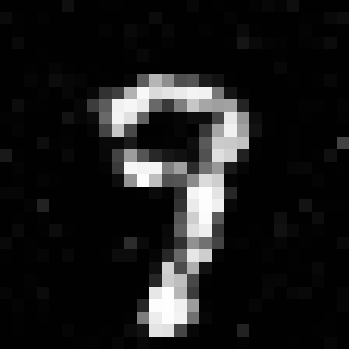
\includegraphics[width=0.3\linewidth]{pic/mnist-res-b.png}
    \caption{生成手写字2}
    \label{mnist-res-b}
\end{figure}

\subsection{正多边形和拼图}
在这两个数据集中间得到数据丧失了重要的细节, 但是保留了对于数据基本观察。
\ref{polygon-res-a}和\ref{polygon-res-b}显示的是正多边形的训练过程中先后抽取的图
片, 从图片中间可以感觉到生成的图片正在趋于形成一个圆形。\ref{tile-res-a}中间生
成的数据观察到数据会划分为两个部分, 但是没有的办法得到可以拼接称为一个图片的数
据。
\begin{figure}[!hbt]
    \centering
    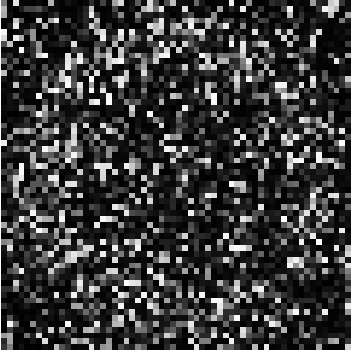
\includegraphics[width=0.3\linewidth]{pic/polygon-res-a.png}
    \caption{正多边形生成结果}
    \label{polygon-res-a}
\end{figure}

\begin{figure}[!hbt]
    \centering
    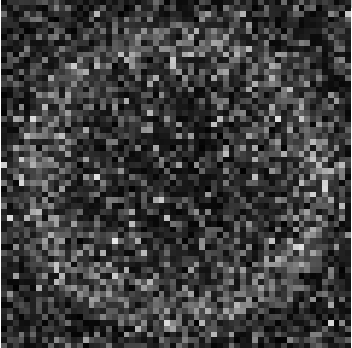
\includegraphics[width=0.3\linewidth]{pic/polygon-res-b.png}
    \caption{正多边形生成结果}
    \label{polygon-res-b}
\end{figure}

\begin{figure}[!hbt]
    \centering
    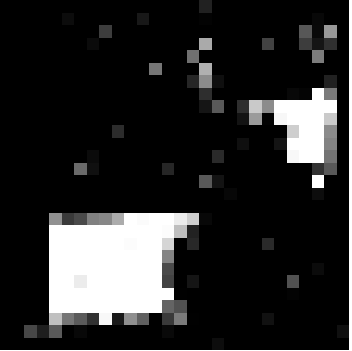
\includegraphics[width=0.3\linewidth]{pic/tile-res-a.png}
    \caption{拼图生成结果}
    \label{tile-res-a}
\end{figure}


\subsection{点和线条}
这两个数据集经过一个晚上的运行,得到的结果依旧是随机造影, 看出来任何重要的信息
。比如\ref{star-res-a}显示的为点图形的结果,该结果中间似乎可以看到点的聚集倾
向, 但是除非看过原始数据才有这一种错觉。
\begin{figure}[!hbt]
    \centering
    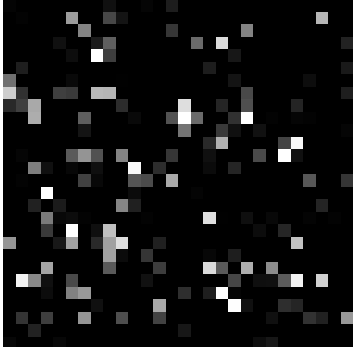
\includegraphics[width=0.3\linewidth]{pic/star-res-a.png}
    \caption{点生成结果,几乎看不到任何结构}
    \label{star-res-a}
\end{figure}
